\setchapterpreamble[u]{\margintoc}
\chapter{Linguaggi e Grammatiche}
\labch{Linguaggi e Grammatiche}




\section{Definizioni fondamentali}

Iniziamo con le definizioni di base che saranno fondamentali in tutto il testo.

Un \textbf{simbolo} o \textbf{carattere} è un qualsiasi elemento.


\begin{definition}\label{def:alfabeto}
Un \keyword{alfabeto}, normalmente indicato con $\Sigma$, è un insieme finito e non vuoto di simboli.
\end{definition}

Esempi di alfabeti sono \texttt{abcdefghijklmnopqrstuvwxyz}, e l'insieme di cifre \texttt{0123456789}.
Siccome un alfabeto è un insieme, l'ordine dei simboli non è rilevante.
In altre parole \texttt{9876543210} è sempre l'alfabeto delle cifre.
Nel seguito useremo $\Sigma_{L}$ per indicare l'alfabeto delle lettere minuscole e
$\Sigma_{C}$ per l'alfabeto delle cifre.


La giustapposizione di simboli permette di creare parole o stringhe, quali ad
esempio \texttt{parola} o \texttt{2301}.

\begin{definition}\label{def:parola}
Sia $\Sigma$ un alfabeto.
Allora una \keyword{parola} è una sequenza $\sigma_{1}\cdots\sigma_{n}$ di simboli, non necessariamente
distinti, dell'alfabeto $\Sigma$.
Una parola viene normalmente rappresentata tramite la giustapposizione dei
simboli che compongono la sequenza, rispettando l'ordine.
\end{definition}

Normalmente usiamo le ultime lettere dell'alfabeto latino (ad esempio $w$, $x$,
$y$, $z$) per rappresentare parole.
La \keyword{lunghezza} di una parola è il numero di simboli nella sequenza.
La lunghezza della parola $z$ viene indicata con $|z|$.

Alcuni simboli sono speciali perchè hanno un significato particolare e non fanno parte di nessun alfabeto $\Sigma$.
Il primo simbolo speciale che vediamo è $\epsilon$ e rappresenta la stringa vuota,
formata dalla sequenza di zero simboli.

\begin{definition}\label{def:linguaggio}
Dato un alfabeto $\Sigma$, un \keyword{linguaggio} $L$ è un insieme di parole su $\Sigma$.
\end{definition}

Sebbene l'alfabeto sia finito, un linguaggio potrebbe contenere un numero
infinito di parole.
Diventa quindi importante capire quando un linguaggio infinito ha una
rappresentazione finita.
Notare che praticamente tutti i linguaggi rilevanti sono infiniti, ma con
rappresentazione finita.
Prendiamo ad esempio JSON: abbiamo una specifica formale (quindi una sequenza di
caratteri corrisponde ad un documento JSON se e solo se soddisfa la specifica),
e l'insieme dei documenti JSON è infinito.

\begin{example}\label{exa:numeri}
Un numero è formato da una parte intera che consiste unicamente di cifre e,
opzionalmente, da una parte frazionaria che consiste unicamente di cifre.
Se la parte frazionaria esiste, allora la parte intera e la parte frazionaria
sono separate da un punto.
La parte intera non può iniziare con \texttt{0} e la parte frazionaria non può
finire con \texttt{0}.
L'insieme di tutti i numeri è un linguaggio (infinito).
\end{example}

La descrizione in \Cref{exa:numeri} è di natura insiemistica:  il
linguaggio è visto come l'insieme delle parole che lo compongono.
Esistono due punti di vista alternativi: (1) considerare come sia possibile generare
tutte le parole di un linguaggio, (2) descrivere una procedura che determini se
una parola appartiene al linguaggio.
Si noti che la definizione di linguaggio non cambia.
Nel seguito vedremo come questi tre punti di vista si complementino e
interagiscono fra loro.
L'ultimo approccio, basato sulla procedura per determinare se una parola
appartiene al linguaggio, ci porta a definire il primo fondamentale problema
computazionale, detto problema dell'\keyword{appartenenza} ad un linguaggio.


\begin{problem}[Appartenenza]\label{pb:appartenenza}
Siano $L$ un linguaggio e $z$ una parola, entrambi sull'alfabeto $\Sigma$.
Determinare se $z$ sia una parola del linguaggio $L$.
\end{problem}

Il problema dell'appartenenza è un problema di \keyword{decisione}, perchè
ammette solo due risposte: sì o no.


\begin{itemize}
	\item si definisce \textbf{potenza di un alfabeto} $\Sigma^k$ come l'insieme di tutte le sequenze (espressi come stringhe e non simboli) di lunghezza $k\in\mathbb{N},\, k>0$ ottenibili da quell'alfabeto (se $\Sigma^2$ si avranno tutte le sequenza di 2 elementi etc...). Se ho $k=1$ si ha $\Sigma^1\neq \Sigma$ in quanto ora ho stringhe e non simboli. Se ho $k=0$ ho $\Sigma^0=\varepsilon$. Dato $k$ ho $|\Sigma|$ che è la cardinalità dell'insieme $\Sigma$ (e non la sua lunghezza come nel caso delle stringhe); sia $w\in\Sigma^k=a_1,a_2,...,a_k,\,a_i\in\Sigma$ e $|\Sigma|=q$ ora: $$|\Sigma^k|=q^k$$
	\item si definisce $\Sigma^*$ come\textbf{ chiusura di Kleene} che è l'unione infinita di $\Sigma^k$ ovvero $$\Sigma*=\Sigma^0\cup \Sigma^1\cup...\cup \Sigma^k$$
	\item si ha che $\Sigma^+$ è l'unione per $k\geq 1$ di $\Sigma^k$ ovvero:
				$$\Sigma+=\Sigma^1\cup \Sigma^2\cup...\cup \Sigma^k= \Sigma^*-\Sigma^0$$
				per esempio, per l'insieme $\{0,1\}$ si ha:
				$$\Sigma^*=\{\varepsilon,0,1,00,01,10,100,000,...\}$$
	\item quindi un \textbf{linguaggio} \textit{L} è un insieme di stringhe e:
				$$L\subseteq \Sigma^*$$
				si hanno sottoinsiemi particolari, come l'insieme vuoto, che resta però un linguaggio, il \textbf{linguaggio vuoto} e $\emptyset\in\Sigma^k,\,|\emptyset|=0$ che è diverso dal linguaggio che contiene la stringa vuota $|\varepsilon|=1$ (che conta come una stringa). Inoltre $\Sigma^*\subseteq \Sigma^*$ che ha lunghezza infinita. Posso concatenare due stringhe con un punto: $a\cdot b\cdot c=abc$ e $a\cdot \varepsilon=a$. Ovviamente la stringa concatenata è lunga come la somma delle lunghezze delle stringhe che la compongono. Vediamo qualche esempio di linguaggio:
				\begin{itemize}
					\item il linguaggio di tutte le stringhe che consistono in $n$ 0 seguiti da $n$ 1:
								$$\{\varepsilon,01,0011,000111,...\}$$
					\item l'insieme delle stringhe con un uguale numero di 0 e di 1:
								$$\{\varepsilon,01,10.0011,0101.1001,..\}$$
					\item l'insieme dei numeri binari il cui valore è un numero primo:
								$$\{\varepsilon,10 , 11, 101, 111,1011,...\}$$
					\item $\Sigma^*$ è un linguaggio per ogni alfabeto $\Sigma$
					\item $\emptyset$, il linguaggio vuoto, e $\{\varepsilon\}$ sono un linguaggio rispetto a qualunque alfabeto
				\end{itemize}
\end{itemize}
Prendiamo un alfabeto $\Sigma=\{0, 1\}$ con la sua chiusura di Kleen $\Sigma=\{0, 1\}^*$. Quando si ha un input si può avere un problema di decisione, \textit{P}, che dia come output "si" o "no". Posso avere un problema di decisione (o \textit{membership}) su $w\in\Sigma=\{0, 1\}^*$, con \textit{w} stringa, che dia in output "si" o "no". Un linguaggio \textit{L} sarà:
$$L=\{w\in\{0, 1\}^*\,|\,\, P(w)=si$$
quindi si ha che:
$$\Sigma^*\backslash L=\{P(w)=no\}$$
Vediamo ora un esempio di \textit{Context Free Language (CFL)}, costruito a partire da una \textit{Context Free Grammar (CFG)}:
\begin{example}
	Sia $\Sigma=\{0, 1\}$ e $L_{pal}="stringhe\,\, palindrome\,\, binarie"$.
	Quindi, per esempio, $0110\in L,\,\, 11011\in L$ ma $10010\not\in L$. Si ha che $\varepsilon$, la stringa vuota, appartiene a $L$. Diamo una definizione ricorsiva:
	\begin{itemize}
		\item \textbf{base:} $\varepsilon,\, 0\,\ 1\in L_{pal}$
		\item \textbf{passo:} se $w$ è palindroma allora $0w0$ è palindromo e $1w1$ è palindromo
	\end{itemize}
	una variabile generica $S$ può sottostare alle \textit{regole di produzione} di una certa grammatica. In questo caso si ha uno dei seguenti:
	$$S\to\varepsilon,\, S\to 0,\, S\to 1,\, S\to 0S0,\, S\to 1S1$$
\end{example}
Si ha che una grammatica $G$ è una quadrupla $G=(V,\,T,\,P,\,S)$ con:
\begin{itemize}
	\item $V$ simboli variabili
	\item $T$ simboli terminali, ovvero i simboli con cui si scrivono le stringhe alla fine
	\item $P$ regole di produzione
	\item $S$ variabile di partenza \textit{start}
\end{itemize}
riprendiamo l'esempio sopra:
\begin{example}
	$$G_{pal}=(V=\{S\},\, T=\{0, 1\},\, P,\, S)$$
	con:
	$$P=\{S\to\varepsilon,\, S\to 0,\, S\to 1,\, S\to 0S0,\, S\to 1S1\}$$
	Si può ora costruire un algoritmo per creare una stringa palindroma a partire dalla grammatica $G$:
	$$\underbrace{S}_{\mbox{start}}\underbrace{\to}_{\mbox{applico una regola}} 1S1 \to 01S10\to \underbrace{01010}_{\mbox{sostituisco variabile}}$$

	con $S,\, 1S1\,\, e\,\, 01S10$ che sono \textit{forme sentenziali}. Posso così ottenere tutte le possibili stringhe. Esiste anche una forma abbreviata:
	$$S\to \varepsilon|o|1|0S0|1S1$$
	Non si fanno sostituzioni in parallelo, prima una $S$ e poi un'altra
\end{example}
%aggiungi esempio parentesi
Si hanno 4 grammatiche formali, \textit{gerarchia di Chomsky}:
\begin{itemize}
	\item \textbf{tipo 0:} non si hanno restrizioni sulle regole di produzione, $\alpha\to\beta$. Sono linguaggi ricorsivamente numerabili e sono rappresentati dalle \textit{macchine di Turing}, deterministiche o non deterministiche (la macchina di Turing è un automa)
	\item \textbf{tipo 1:}  il lato destro della produzione ha lunghezza almeno uguale a quello sinistro. Sono grammatiche dipendenti dal contesto (\textit{contestuali}) e come automa hanno\textit{ la macchina di Turing che lavora in spazio lineare}:
				$$\alpha_1A\alpha_2\to \alpha_1B\alpha_2$$
				con $\alpha_1$ e $\alpha_2$ detti \textit{contesto} e $\alpha_1,\,\alpha_2,\, \beta\in (V\cup T)^*$
	\item \textbf{tipo 2:} sono quelle libere dal contesto, context free. Come regola ha $A\to\beta$ con $A\in V$ e $\beta\in (V\cup T)^*$ e come automa ha gli \textit{automi a pila non deterministici}
	\item \textbf{tipo 3:} sono le grammatiche \textit{regolari}. Come regole ha $A\to\alpha B$ (o $A\to B\alpha$) e $A\to\alpha$  con $A,B\in V$ e $\alpha\in T$. Come automi ha gli \textit{automi a stato finito deterministici o non deterministici}
\end{itemize}
%aggiungi esercizio
\newpage
\begin{example}
	Sia $G=(V,T,O,E)$, con $V=\{E,I\}$ e $T=\{a,b,0,1,(,),+,*\}$
	quindi ho le seguenti regole, è di tipo 3:
	\begin{enumerate}
		\item $E\to I$
		\item $E\to E+E$
		\item $E\to E*E$
		\item $E\to (E)$
		\item $I\to a$
		\item $I\to b$
		\item $I\to Ia$
		\item $I\to Ib$
		\item $I\to I0$
		\item $I\to I1$
	\end{enumerate}
	voglio ottenere $a*(a+b00)$
	sostituisco sempre a destra (right most derivation)
	$$E\to E*E\to E*(E)\to E*(E+E)\to E*(E+I)\to E+(E+I0)$$
	$$\to R+(I+b00)\to E*(a+b00)\to I*(a+b00)\to a*(a+b00)$$

	usiamo ora \textit{l'inferenza ricorsiva}:
	\begin{center}
		\begin{tabular}{|c|c|c|c|c|}
			\hline
			passo & stringa ricorsiva & var & prod & passo stringa impiegata \\
			1     & a                 & I   & 5    & $\backslash$            \\
			\hline
			2     & b                 & I   & 6    & $\backslash$            \\
			\hline
			3     & b0                & I   & 9    & 2                       \\
			\hline
			4     & b00               & I   & 9    & 3                       \\
			\hline
			5     & a                 & E   & 1    & 1                       \\
			\hline
			6     & b00               & E   & 1    & 4                       \\
			\hline
			7     & a+b00             & E   & 2    & 5,6                     \\
			\hline
			8     & (a+b00)           & E   & 4    & 7                       \\
			\hline
			9     & a*(a+b00)         & E   & 3    & 5, 8                    \\
			\hline
		\end{tabular}
	\end{center}
\end{example}
definisco formalmente la derivazione $\to$:
\begin{definition}
	Prendo una grammatica $G=(V,T,P,S)$, grammatica CFG. Se $\alpha A \beta$ è una stringa tale che $\alpha,\beta\in (V\cup T)^*$, appartiene sia a variabili che terminali. Sia $A\in V$ e sia $a\to \gamma$ una produzione di $G$. Allora
	scriviamo:
	$$\alpha A \beta \to \alpha\gamma\beta$$
	con $\gamma\in (V\cup T)^*$.\\
	Le sostituzioni si fanno indipendentemente da $\alpha$ e $\beta$.
	Questa è quindi la definizione di derivazione.
\end{definition}
\begin{definition}
	Definisco il simbolo $\to _*$, ovvero il simbolo di \textit{derivazioni in 0 o più passi}. Può essere definito in modo ricorsivo. Per induzione sul numero di passi.
	\begin{itemize}
		\item la base dice che  $\forall \alpha\in (V\cup T)^*,\, \alpha\to * \,\alpha$
		\item il passo è: se $\alpha\to_{G_*} \,\beta $ e $ \beta \to_{G_*} \,\gamma$ allora $\alpha\to_* \,\gamma$
	\end{itemize}
	Si può anche dire che $\alpha\to_{G_*}\, \beta$ sse esiste una sequenza di stringhe $\gamma_1,...,\gamma_n$ con $n\geq 1$ tale che $\alpha=\gamma_1$, $\beta=\gamma_n$ e $\forall i,\, 1<i<n-1$ si ha che $\gamma_1\to \gamma_{i+1}$
	la derivazione in 0 o più passi è la chiusura transitiva della derivazione
\end{definition}
\begin{definition}
	avendo ora definito questi simboli possiamo definire una forma sentenziale. Infatti è una stringa $\alpha$ tale che:
	$$\forall \alpha\in (V\cup T)^* \mbox{ tale che }S\to_{G_*}\, \alpha$$
\end{definition}
\begin{definition}
	data $G=(V,T,P,S)$ si ha che $L(G)=\{w\in T^* |\, S\to_{G_*}\, w\}$ ovvero composto da stringhe terminali che sono derivabili o 0 o più passi.
\end{definition}
\begin{example}
	formare una grammatica CFG per il linguaggio:
	$$L=\{0^n 1^n| n\geq 1\}=\{01, 0011, 000111,...\}$$
	con $x^n$ intendo una concatenazione di $n$ volte $x$ (che nel nostro caso sono 0 e 1).\\
	posso scrivere:
	$$0^n 1^n =00^{n-1} 1^{n-1}1$$
	il nostro caso base sarà la stringa $01$, Poi si ha:
	$G=(V,T,P,S)$, $T=\{0,1\}$, $V=\{S\}$, il caso base $S\to 01$  e $S\to 0S1$
	il caso passo è quindi: se $w= 0^{n-1}1^{n-1}\in L$ allora $0w1\in L$.\\
	Ora voglio dimostare che $000111\in L$, ovvero $S\to*\, 000111$:\\
	$$S\to\, 0S1 \to 00S11\to 000S111$$
\end{example}
\begin{theorem}
	data la grammatica $G=\{V,T,P,S)$ CFG e $\alpha\in (V\cup T)^*$. Si ha che vale $S\to_*\, \alpha$ sse $S\to_{lm_*}\, \alpha$ sse $S\to_{rm_*}\, \alpha$. Con $\to_{lm_*}$ simbolo di \textit{left most derivation }e $\to_{rm_*}$ simbolo di \textit{right most derivation}
\end{theorem}
\begin{example}
	formare una grammatica CFG per il linguaggio:
	$$L=\{0^n 1^n| n\geq 0\}=\{\varepsilon, 01, 0011, 000111,...\}$$
	stavolta abbiamo anche la stringa vuota. Il caso base stavolta è $S\to\varepsilon| \, 0S1$
\end{example}
\begin{example}
	Fornisco una CFG per $L=\{a^n|n\geq 1\}=\{a, aa, aaa,...\}$.
	La base è $a$ \\il passo è che se $a^{n-1}\in L$ allora $a^{n-1}a\in L$ ( o che $aa^{n-1}\in L$).\\
	Si ha la grammatica $G=\{V,T,P,S)$, $V=\{S\}$, $T=\{a\}$ e si hanno $S\to a|\,Sa$ (o  $S\to a|\,aS$). Dimostro che $a^3\in L$.
	$$S\to Sa \to Saa\to aaa$$
	oppure
	$$S\to aS\to aaS\to aaa$$
\end{example}
\begin{example}
	trovo una CFG per $L=\{(ab)^n|n\geq 1\}=\{ab, abab, ababab,...\}$\\
	La base è $ab$ \\il passo è che se $(ab)^{n-1}\in L$ allora $(ab)^{n-1}ab\in L$.\\
	Si ha la grammatica $G=\{V,T,P,S)$, $V=\{S\}$, $T=\{a,b\}$ (anche se in realtà $T=\{ab\}$) e si hanno $S\to ab|\,Aab$. Poi dimostro come l'esempio sopra
\end{example}
\begin{example}
	trovo una CFG per $L=\{a^n c b^n|n\geq 1\}=acb,aacbb,aaacbbb,...\}$\\
	Il caso base è $acb$ il passo è che se $a^{n-1}cb^{n-1}\in L$ allora $a^{n-1}cb^{n-1}acb\in L$
	Si ha la grammatica $G=\{V,T,P,S)$, $V=\{S\}$, $T=\{a,b,c\}$ e si hanno $S\to aSb|acb$.\\
	dimostro che $aaaacbbbbb\in L$:
	$$S\to aSb\to aaSbb\to aaaaSbbb\to aaaacbbbb$$

	provo a usare anche una grammatica regolare, con le regole $S\to aS|c$, $c\to cB$ e $B\to bB|b$;
	$$S\to aS\to aaS\to aaC\to aacB\to aacb...$$
	non si può dimostrare in quanto non si può imporre una regola adatta
\end{example}
\begin{example}
	$L=\{a^n c b^{n-1}|n\geq 2\}$, con $a^n c b^{n-1}=a^{n-1}acb^{n-1}$. $S\to aSb|aacb$. Quindi:
	$$S\to aSb\to aaaccbb\in L$$
\end{example}
\begin{example}
	cerco CFG per $L=\{a^n c^k b^n|\,n,\,k>0\}$. $a$ e $b$ devono essere uguali, uso quindi una grammatica context free, mentre $c$ genera un linguaggio regolare.\\
	Si ha la grammatica $G=\{V,T,P,S)$, $V=\{S,C\}$, $T=\{a,b,c\}$ e si hanno $S\to aSb|aCb$ e $C\to cC|c$. dimostro che $aaaccbbb\in L, n=3,\, k=2$:
	$$S\to aSb \to aaSbb\to aaaCbbb\to aaacCbbb\to aaaccbbb$$
\end{example}
\begin{example}
	scrivere CFG per $L=\{a^nb^nc^kb^k|\, n,\,k\geq 0\}
	$
	$$=\{w\in\{a,b,c,d\}^*|\,a^nb^nc^kb^k|\, n,\,k\geq 0\}$$
	quindi L concatena due linguaggi $L1$ e $L2$, $X=\{a^nb^n\}$ e $Y=\{c^kd^k\}$:
	$$X\to aXb | \varepsilon$$
	$$Y\to cYd | \varepsilon$$
	$$S\to XY$$
	voglio derivare $abcd$:
	$$S\to XY \to XcYd\to aXbcYd\to aXbc\varepsilon d\to a\varepsilon bc\varepsilon d\to abcd$$
	voglio derivare $cd$
	$$S\to XY\to Y\to cYd\to cd$$
\end{example}
Quindi se ho $w\in L1, L2$, ovvero appartenente ad una concatenazione di linguaggi prima uso le regole di un linguaggio, poi dell'altro e infine ottengo il risultato finale.\\
\begin{example}
	scrivere CFG per $L=\{a^nb^kc^kd^n|\, n>0,\, k\geq 0\}
	$.
	$$S\to aSd|\, aXd$$
	$$X\to bXc| \varepsilon$$
	derivo $aabcdd$:
	$$S\to aSd\to aaXdd\to aabXcdd\to aabcdd$$
\end{example}
\begin{example}
	scrivere CFG per $L=\{a^ncb^nc^mad^m|\, n>0,\, m\geq 1\}
	$.
	$$S\to XY$$
	$$X\to aXb|c$$
	$$Y\to cUd| cad$$
	$$S\to XY\to cY\to ccad$$
\end{example}
\begin{example}
	scrivere CFG per $L=\{a^{n+m}xc^nyd^m|\, n,\, m\geq 0\}
	$. $a^{n+m}=a^na^m \mbox{ o } a^ma^n$. Si hanno 2 casi:
	\begin{enumerate}
		\item $L=\{a^na^m xc^nyd^m|\, n,\, m\geq 0\}
					$
		\item $L=\{a^ma^n xc^nyd^m|\, n,\, m\geq 0\}
					$
	\end{enumerate}
	ma solo  $L=\{a^ma^n xc^nyd^m|\, n,\, m\geq 0\}
	$ può generare una CFG (dove non si possono fare incroci, solo concatenazioni e inclusioni/innesti).
	$$S\to aSd| Y$$
	$$Y\to Xy$$
	$$X\to aXc|x$$
	si può fare in 2:
	$$S\to aSd| Xy$$
	$$X\to aXc|x$$
	derivo con $m=n=1$, $aaxcyd$:
	$$S\to aSd\to aXyd\to aaXcyd\to aaxcyd$$
\end{example}
\begin{example}
	scrivere CFG per $L=\{a^nb^m|\, n\geq m \geq 0\}
	$.$$L=\{\varepsilon, a, ab, aa, aab, aabb, aaa, aaab, aaabb, aaabbb,...\}$$
	Se $n\geq m$ allora $\exists k\geq 0 \to n=m+k$. Quindi:
	$$l=\{a^{m+k}b^m|m,k\geq0\}$$ si può scrivere in 2 modi:
	\begin{enumerate}
		\item $l=\{a^ma^kb^m|m,k\geq0\}$ quindi con innesto
		\item $l=\{a^ka^mb^m|m,k\geq0\}$quindi con concatenazione
	\end{enumerate}
	entrambi possibili per una CFG:
	\begin{enumerate}
		\item
					$$S\to XY$$
					$$X\to aX|\varepsilon \mbox{ si può anche scrivere } X\to Xa|\varepsilon$$
					$$Y\to aYb|\varepsilon$$
					oppure
					$$S\to aS|X$$
					$$X\to aXb| \varepsilon$$
		\item
					$$S\to aSb|\varepsilon$$
					$$X\to aX|\varepsilon$$
	\end{enumerate}
\end{example}
\begin{example}
	scrivere CFG per $L=\{a^nb^{m+n}c^h|\, m>h\geq0,\, n\geq0\}
	$.\\
	Se $n>h$ allora $\exists k \to n= h+k$, quindi:
	$$L=\{a^nb^{m+h+k}c^h|\, m>h\geq0,\, n\geq0\}$$. ovvero:
	$$L=\{a^nb^nb^kb^hc^h|\, m\geq 0, k>0, h\geq 0\}$$
	si ha:
	$$S\to XYZ$$
	$$X\to aXb|\varepsilon$$
	$$Y\to Yb|b$$
	$$Z\to bZc|\varepsilon$$
	si può anche fare:
	$$S\to XY$$
	$$X\to aXb|\varepsilon$$
	$$Y\to bYc|Z$$
	$$Z\to bZ|b$$
\end{example}
\begin{example}
	scrivere CFG per $L=\{a^nb^mc^k|\, k>n+m,\, n,m\geq 0\}
	$.\\
	per $n=m=0,\, k=1$ avrò la stringa $c$.
	se $k>n+m$ allora $\exists l>0\to k=n+m+l$ quindi:
	$$L=\{a^nb^mc^{n+m+l}|\, l>0,\, n,m\geq 0\}
	$$
	$$=L=\{a^nb^mc^nc^mc^l|\, l>0,\, n,m\geq 0\}$$
	sistemando:
	$$=L=\{a^nb^mc^lc^mcnl|\, l>0,\, n,m\geq 0\}$$
	quindi:
	$$S\to aSc|X$$
	$$X\to bXc|Y$$
	$$Y\to cY|c$$
\end{example}
\newpage
\begin{example}
	scrivere CFG per $L=\{a^nxc^{n+m}y^hz^kd^{m+h}|\, n,m,k,h\geq 0\}
	$.\\
	ovvero:
	$$L=\{a^nxc^nc^my^hz^kd^hd^m|\, n,m,k,h\geq 0\}$$
	quindi avrò:
	$$S\to XY$$
	$$X\to aXc|x$$
	$$Y\to cYd|W$$
	$$W\to yWd|X$$
	$$Z\to zZ|\varepsilon$$
\end{example}
\begin{example}
	vediamo un esempio di grammatica dipendente dal contesto:
	$$L=\{a^nb^nc^n|\, n\geq 1\}$$
	$G=\{V,T,P,S\}=\{(S,B,C,X)\}=\{(a,b,c),P,S\}$
	ecco le regole di produzione (qui posso scambiare variabili a differenza delle context free):
	\begin{enumerate}
		\item $S\to aSBC$
		\item $S\to aBC$
		\item $CB\to XB$
		\item $XB\to XC$
		\item $XC\to BC$
		\item $aB\to ab$
		\item $bB\to bb$
		\item $bC\to bc$
		\item $cC\to cc$
	\end{enumerate}
	vediamo un esempio di derivazione:
	per $n=1$ ho $abc$ ovvero:
	$$S\to aBC\to abC\to abc$$
	con $n=2$ ho $aabbcc$:
	$S\to aSBC\to aaBCBC\to aaBXBC\to aaBXCC\to aaBBCC\to aabBCC\to aabbCC\to aabbcC\to aabbcc$\\
	%vedere dimostrazione pag 14 soligo
\end{example}
\newpage
\begin{example}
	vediamo un esempio di grammatica dipendente dal contesto:
	$$L=\{a^nb^mc^nd^m|\, n,m\geq 1\}$$
	Si ha:
	$$G=(\{S,X,C,D,Z\},\{a,b,c,d\},P,S)$$
	con le seguenti regole di produzione:
	\begin{itemize}
		\item $S\to aSc|\, aXc$
		\item $X\to bXD|\, bD$
		\item $DC\to CD$
		\item $DC\to DZ$
		\item $DZ\to CZ$
		\item $XZ\to CD$
		\item $bC\to bc$
		\item $cC\to cc$
		\item $cD\to cd$
		\item $dD\to dd$
	\end{itemize}
	provo a derivare $aabbbccddd$ quindi con $n=2,\,m=3$:\\
	$$S\to aSC\to aaXCC\to aabXDCC\to aabbXDDCC\to $$
	$$aabbbDDDCC\to aabbbCCDDD\to aabbbccddd$$
\end{example}
\begin{example}
	Sia $L=\{w\in\{a,b\}^*|\, \mbox{ w contiene lo stesso numero di a e b}\}$:
	$$S\to aSbS|\,bSaS|\, \varepsilon$$
	dimostro per induzione che è corretto:
	\begin{itemize}
		\item \textbf{caso base:} $|w|=0\to w=\varepsilon$
		\item \textbf{caso passo:} si supponga che $G$ produca tutte le stringhe (di lunghezza $<$ di $n$) di $\{a,b\}^*$ con lo stesso numero di \textit{a} e \textit{b} e dimostro che produce anche quelle di lunghezza $n$, sia:
					$$w\in \{a,b\}^* \mid\, |w|=n \mbox{ con\textit{ a} e \textit{b} in egual numero, }m(a)=m(b) \mbox{ con m() che indica il numero di caratteri}$$
					quindi si ha che:
					$$w=aw_1bw_2\mbox{ o } w=bw_1aw_2$$
					sia.
					$$k_1=m(a)\in w_1=m(b)\in w_1$$
					$$k_2=m(a)\in w_2=m(b)\in w_2$$
					allora:
					$$k_1+k_2+1=m(a)\in w= m(b)\in W$$
					sapendo che $|w_1|<n$ e $|w_2|<n$ allora $w_1$ e $w_2$ sono egnerati da G per ipotesi induttiva
	\end{itemize}
\end{example}

\section{Alberi Sintatici}
\begin{definition}
	Data una grammatica CFG, $G=\{V,T,P,S\}$ un \textbf{albero sintattico} per $G$ soddisfa le seguenti condizioni:
	\begin{itemize}
		\item ogni nodo interno è etichettato con una variabile in $V$
		\item ogni foglia è anch'essa etichettata con una variabile o col simbolo di terminale T o con la stringa vuota $\varepsilon$ (in questo caso la foglia è l'unico figlio del padre)
		\item se un nodo interno è etichettato con A i suoi figli saranno etichettati con X1, ..., Xk e $A\to  X1, ..., Xk$ sarà una produzione di $G$ in $P$. Se un $X_i$ è $\varepsilon$ sarà l'unica figlio e $A\to \varepsilon$ sarà comunque una produzione di $G$
	\end{itemize}
	La concatenazione in ordine delle foglie viene detto \textbf{prodotto dell'albero}
\end{definition}
\newpage
\begin{example}
	Usiamo l'esempio delle stringhe palindrome:
	$$P\to 0P0|\,1P1|\varepsilon$$
	sia il seguente albero sintatico:
	\begin{center}
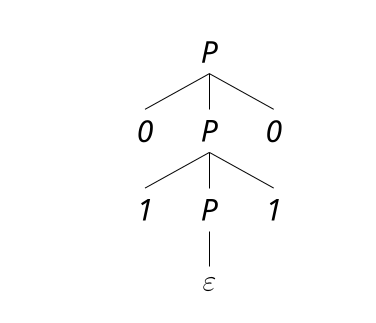
\includegraphics{example_1.1.1.png
}
%		\psframebox[linestyle=none,framesep=10pt]{%
%			\pstree{\LFTw{t}{\fontspec{Noto Sans}[Script=Latin]P}}{\pstree{\Tp[edge=none]}{%
%					\LFTw{t}{\fontspec{Noto Sans}[Script=Latin]0}
%					\pstree{\LFTw{t}{\fontspec{Noto Sans}[Script=Latin]P}}{\pstree{\Tp[edge=none]}{%
%							\LFTw{t}{\fontspec{Noto Sans}[Script=Latin]1}
%							\pstree{\LFTw{t}{\fontspec{Noto Sans}[Script=Latin]P}}{\pstree{\Tp[edge=none]}{%
%									\LFTw{t}{\fontspec{Noto Sans}[Script=Latin]$\varepsilon$}}}
%							\LFTw{t}{\fontspec{Noto Sans}[Script=Latin]1}}}
%					\LFTw{t}{\fontspec{Noto Sans}[Script=Latin]0}}}}
	\end{center}
\end{example}
\begin{example}
	Si ha:
	$$E\to I|\, E+E|\, E*E|\, (E)$$
	$$I\to a|\,b|\,Ia|\,Ib|\,I0|\,I1$$
	un albero sintattico per $a*(a+b00)$ può essere:
	\begin{center}
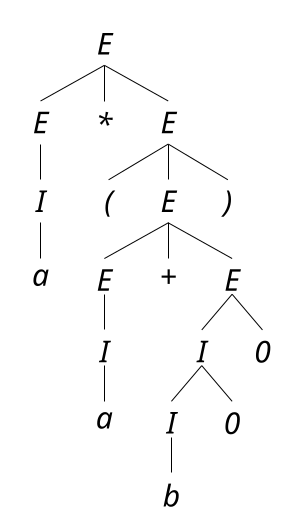
\includegraphics{example_1.1.2.png}
%		\psframebox[linestyle=none,framesep=10pt]{%
%			\pstree{\LFTw{t}{\fontspec{Noto Sans}[Script=Latin]E}}{\pstree{\Tp[edge=none]}{%
%					\pstree{\LFTw{t}{\fontspec{Noto Sans}[Script=Latin]E}}{\pstree{\Tp[edge=none]}{%
%							\pstree{\LFTw{t}{\fontspec{Noto Sans}[Script=Latin]I}}{\pstree{\Tp[edge=none]}{%
%									\LFTw{t}{\fontspec{Noto Sans}[Script=Latin]a}}}}}
%					\LFTw{t}{\fontspec{Noto Sans}[Script=Latin]*}
%					\pstree{\LFTw{t}{\fontspec{Noto Sans}[Script=Latin]E}}{\pstree{\Tp[edge=none]}{%
%							\LFTw{t}{\fontspec{Noto Sans}[Script=Latin](}
%								\pstree{\LFTw{t}{\fontspec{Noto Sans}[Script=Latin]E}}{\pstree{\Tp[edge=none]}{%
%										\pstree{\LFTw{t}{\fontspec{Noto Sans}[Script=Latin]E}}{\pstree{\Tp[edge=none]}{%
%												\pstree{\LFTw{t}{\fontspec{Noto Sans}[Script=Latin]I}}{\pstree{\Tp[edge=none]}{%
%														\LFTw{t}{\fontspec{Noto Sans}[Script=Latin]a}}}}}
%										\LFTw{t}{\fontspec{Noto Sans}[Script=Latin]+}
%										\pstree{\LFTw{t}{\fontspec{Noto Sans}[Script=Latin]E}}{\pstree{\Tp[edge=none]}{%
%												\pstree{\LFTw{t}{\fontspec{Noto Sans}[Script=Latin]I}}{\pstree{\Tp[edge=none]}{%
%														\pstree{\LFTw{t}{\fontspec{Noto Sans}[Script=Latin]I}}{\pstree{\Tp[edge=none]}{%
%																\LFTw{t}{\fontspec{Noto Sans}[Script=Latin]b}}}
%														\LFTw{t}{\fontspec{Noto Sans}[Script=Latin]0}}}
%												\LFTw{t}{\fontspec{Noto Sans}[Script=Latin]0}}}}}
%								\LFTw{t}{\fontspec{Noto Sans}[Script=Latin])}}}}}}
	\end{center}
\end{example}
\newpage
Data una CFG si ha che i seguenti cinque enunciati si equivalgono:
\begin{enumerate}
	\item la procedura di inferenza ricorsiva stailisce che una stringa $w$ di simboli terminali appartiene al linguaggio $L(A)$ con $A$ variabile
	\item $A\to ^*w$
	\item $A\to^*_{lm}w$
	\item $A\to^*_{rm}w$
	\item esiste un albero sintattico con radice $A$ e prodotto $w$
\end{enumerate}
queste 5 proposizioni si implicano l'uni l'altra:
\begin{center}
	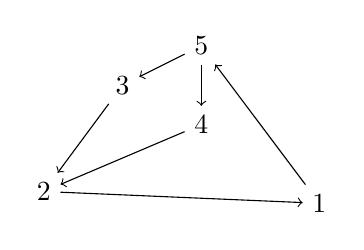
\begin{tikzpicture}
		\node (top) at (0,0) {5};
		\node (a) at(-1,-0.5) {3};
		\node (b) at(0,-1) {4};
		\node (c) at(-2.0,-1.85) {2};
		\node (d) at(1.5,-2) {1};
		\draw [->] (top) -- (a);
		\draw [->] (top) -- (b);
		\draw [->] (a) -- (c);
		\draw [->] (b) -- (c);
		\draw [->] (c) -- (d);
		\draw [->] (d) -- (top);
	\end{tikzpicture}
\end{center}
vediamo qualche dimostrazione di implicazione tra queste proposizioni:
\begin{proof}[da 1 a 5]
	si procede per induzione:
	\begin{itemize}
		\item \textbf{caso base:} ho un livello solo (una sola riga), $\exists A\to w$:
					$$\overset{A}{\overset{\triangle}w}$$
		\item \textbf{caso passo:} suppongo vero per un numero di righe $\leq n$, lo dimsotro per $n+1$ righe:
					$$A\to X_1,X_2,...,X_k$$
					$$w=w_1,w_2,...,w_k$$
					ovvero, in meno di $n+1$ livelli:
					\begin{center}
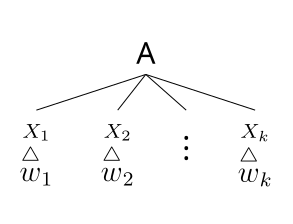
\includegraphics{caso_passo.png}
					% \psframebox[linestyle=none,framesep=10pt]{%
%				      \pstree{\LFTw{t}{\fontspec{Noto Sans}[Script=Latin]A}}{\pstree{\Tp[edge=none]}{%
%						      \LFTw{t}{\fontspec{Noto Sans}[Script=Latin]$\overset{X_1}{\overset{\triangle}w_1}$}
%						      \LFTw{t}{\fontspec{Noto Sans}[Script=Latin]$\overset{X_2}{\overset{\triangle}w_2}$}
%						      \LFTw{t}{\fontspec{Noto Sans}[Script=Latin]$\vdots$}
%						      \LFTw{t}{\fontspec{Noto Sans}[Script=Latin]$\overset{X_k}{\overset{\triangle}w_k}$}}}}
					\end{center}
	\end{itemize}
\end{proof}
\begin{proof}[da 5 a 3]
	procedo per induzione:
	\begin{itemize}
		\item \textbf{caso base (n=1): }$\exists A\to w\mbox{ quindi } A\to_{lm}w$, come prima si ha un solo livello:
					$$\overset{A}{\overset{\triangle}w}$$
		\item \textbf{caso passo: }suppongo che la proprierà valga per ogni albero di profondità minore uguale a $n$, dimostro che valga per gli alberi profondi $n+1$:
					$$A\to X_1,X_2,...,X_k$$
					$$w=w_1,w_2,...,w_k$$
					ovvero, in meno di $n+1$ livelli:
					\begin{center}
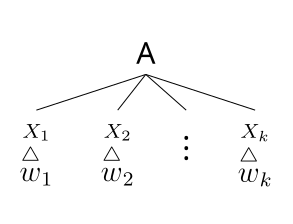
\includegraphics{caso_passo.png}
%			      \psframebox[linestyle=none,framesep=10pt]{%
%				      \pstree{\LFTw{t}{\fontspec{Noto Sans}[Script=Latin]A}}{\pstree{\Tp[edge=none]}{%
%						      \LFTw{t}{\fontspec{Noto Sans}[Script=Latin]$\overset{X_1}{\overset{\triangle}w_1}$}
%						      \LFTw{t}{\fontspec{Noto Sans}[Script=Latin]$\overset{X_2}{\overset{\triangle}w_2}$}
%						      \LFTw{t}{\fontspec{Noto Sans}[Script=Latin]$\vdots$}
%						      \LFTw{t}{\fontspec{Noto Sans}[Script=Latin]$\overset{X_k}{\overset{\triangle}w_k}$}}}}
					\end{center}
					$$A\to_{lm} X_1,X_2,...,X_k$$
					$$x_1\to^*_{lm}w_1 \mbox{ per ipotesi induttiva si ha un albero al più di n livelli}$$
					quindi:
					$$A\to_{lm}X_1,...,X_k\to^*_{lm}w_1,X_2,...,X_k\to^*_{lm}...\to^*_{lm}w_1,...,w_k=w$$
	\end{itemize}
	\begin{example}
		$$E\to I\to Ib\to ab$$
		$$\alpha E\beta\to\alpha I\beta\to \alpha Ib\beta\to \alpha ab\beta,\,\,\,\alpha,\beta\in(V\cup T)^*$$
	\end{example}
\end{proof}
\begin{example}
	Mostro l'esistenza di una derivazione sinistra dell'albero sintattico di $a*(a+b00)$:
	$$E\to^*_{lm}E*E\to^*_{lm}I*E\to^*_{lm}a*E\to^*_{lm}a*(E)\to^*_{lm}a*(E+E)\to^*_{lm}$$
	$$a*(I+E)\to^*_{lm}a*(a+E)\to^*_{lm}a*(a+I)\to^*_{lm}a+(a+I0)\to^*_{lm}a*(a+I00)\to^*_{lm}a*(a+b00)$$
\end{example}
\section{Grammatiche ambigue}
\begin{definition}
	Una grammatica è definita ambigua se esiste una stringa $w$ di terminali che ha più di un albero sintattico
\end{definition}
\begin{example}
	vediamo un esempio:
	\begin{enumerate}
		\item $E\to E+E\to E+E*E$
					ovvero:
					\begin{center}
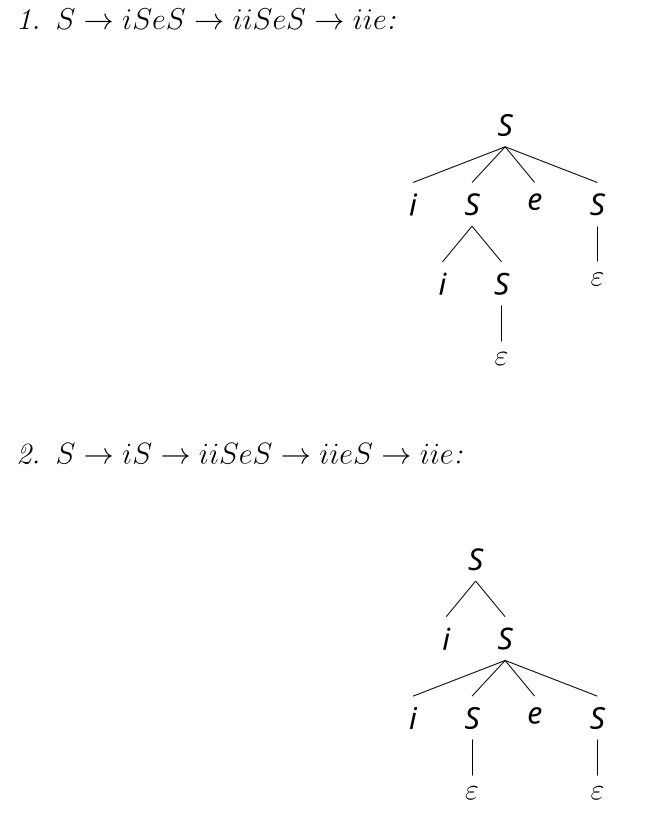
\includegraphics{ambigua1.png}
%			      \psframebox[linestyle=none,framesep=10pt]{%
%				      \pstree{\LFTw{t}{\fontspec{Noto Sans}[Script=Latin]E}}{\pstree{\Tp[edge=none]}{%
%						      \LFTw{t}{\fontspec{Noto Sans}[Script=Latin]E}
%						      \LFTw{t}{\fontspec{Noto Sans}[Script=Latin]+}
%						      \pstree{\LFTw{t}{\fontspec{Noto Sans}[Script=Latin]E}}{\pstree{\Tp[edge=none]}{%
%								      \LFTw{t}{\fontspec{Noto Sans}[Script=Latin]E}
%								      \LFTw{t}{\fontspec{Noto Sans}[Script=Latin]*}
%								      \LFTw{t}{\fontspec{Noto Sans}[Script=Latin]E}}}}}}
					\end{center}
		\item $E\to E*E\to E+E*E$
					ovvero:
					\begin{center}
%			      \psframebox[linestyle=none,framesep=10pt]{%
%				      \pstree{\LFTw{t}{\fontspec{Noto Sans}[Script=Latin]E}}{\pstree{\Tp[edge=none]}{%
%						      \pstree{\LFTw{t}{\fontspec{Noto Sans}[Script=Latin]E}}{\pstree{\Tp[edge=none]}{%
%								      \LFTw{t}{\fontspec{Noto Sans}[Script=Latin]E}
%								      \LFTw{t}{\fontspec{Noto Sans}[Script=Latin]+}
%								      \LFTw{t}{\fontspec{Noto Sans}[Script=Latin]E}}}
%						      \LFTw{t}{\fontspec{Noto Sans}[Script=Latin]*}
%						      \LFTw{t}{\fontspec{Noto Sans}[Script=Latin]E}}}}
					\end{center}
	\end{enumerate}
	si arriva a due stringhe uguali ma con alberi diversi. Introduciamo delle categorie sintatiche, dei vincoli alla produzione delle regole:
	\begin{enumerate}
		\item $E\to T|\, E+T$
		\item $T\to F|\, T+F$
		\item $F\to I|\, (E)$
		\item $I\to a|\,b|\,Ia|,Ib|\,I0|\,I1$
	\end{enumerate}
\end{example}
Possono esserci più derivazioni di una stringa ma l'importante è che non ci siano alberi sintattici diversi. Capire se una CFG è ambigua è un problema indecidibile
\begin{example}
	vediamo un esempio:
	$$S\to \varepsilon|\,SS|\, iS|\, iSeS$$
	con S=statement, i=if e e=else. Considero due derivazioni:
	\begin{enumerate}
		\item $S\to iSeS\to iiSeS\to iie$:
					\begin{center}
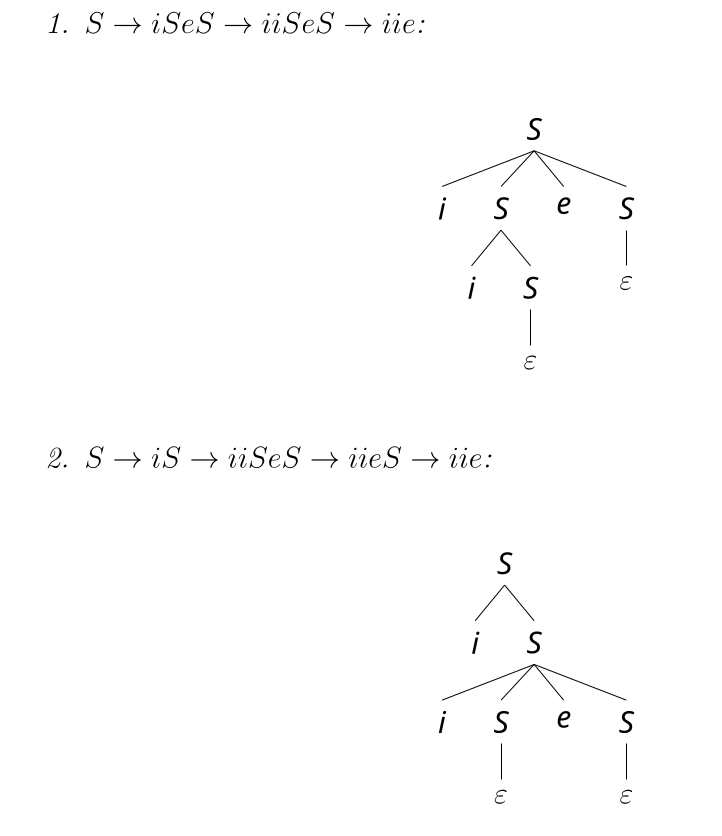
\includegraphics{ambigua2.png}

%			      \psframebox[linestyle=none,framesep=10pt]{%
%				      \pstree{\LFTw{t}{\fontspec{Noto Sans}[Script=Latin]S}}{\pstree{\Tp[edge=none]}{%
%						      \LFTw{t}{\fontspec{Noto Sans}[Script=Latin]i}
%						      \pstree{\LFTw{t}{\fontspec{Noto Sans}[Script=Latin]S}}{\pstree{\Tp[edge=none]}{%
%								      \LFTw{t}{\fontspec{Noto Sans}[Script=Latin]i}
%								      \pstree{\LFTw{t}{\fontspec{Noto Sans}[Script=Latin]S}}{\pstree{\Tp[edge=none]}{%
%										      \LFTw{t}{\fontspec{Noto Sans}[Script=Latin]$\varepsilon$}}}}}
%						      \LFTw{t}{\fontspec{Noto Sans}[Script=Latin]e}
%						      \pstree{\LFTw{t}{\fontspec{Noto Sans}[Script=Latin]S}}{\pstree{\Tp[edge=none]}{%
%								      \LFTw{t}{\fontspec{Noto Sans}[Script=Latin]$\varepsilon$}}}}}}\end{center}
%		\item $S\to iS\to iiSeS\to iieS\to iie$:
%		      \begin{center}
%
%			      \psframebox[linestyle=none,framesep=10pt]{%
%				      \pstree{\LFTw{t}{\fontspec{Noto Sans}[Script=Latin]S}}{\pstree{\Tp[edge=none]}{%
%						      \LFTw{t}{\fontspec{Noto Sans}[Script=Latin]i}
%						      \pstree{\LFTw{t}{\fontspec{Noto Sans}[Script=Latin]S}}{\pstree{\Tp[edge=none]}{%
%								      \LFTw{t}{\fontspec{Noto Sans}[Script=Latin]i}
%								      \pstree{\LFTw{t}{\fontspec{Noto Sans}[Script=Latin]S}}{\pstree{\Tp[edge=none]}{%
%										      \LFTw{t}{\fontspec{Noto Sans}[Script=Latin]$\varepsilon$}}}
%								      \LFTw{t}{\fontspec{Noto Sans}[Script=Latin]e}
%								      \pstree{\LFTw{t}{\fontspec{Noto Sans}[Script=Latin]S}}{\pstree{\Tp[edge=none]}{%
%										      \LFTw{t}{\fontspec{Noto Sans}[Script=Latin]$\varepsilon$}}}}}}}}
					\end{center}
	\end{enumerate}
	Si ha quindi una grammatica ambigua
\end{example}
\begin{theorem}
	Per ogni CFG, con $G=(V, T, P, S)$, per ogni stringa $w$ di terminali si ha che $w$ ha due alberi sintattici distinti sse ha due derivazioni sinistre da S distinte.\\
	Se la grammatica non è ambigua allora esiste un'unica derivazione sinistra da $S$
\end{theorem}
\subsubsection{Linguaggi inerentemente ambigui}
\begin{definition}
	Un linguaggio $L$ è inerentemente ambiguo se tutte le grammatiche CFG per tale linguaggio sono a loro volta ambigue
\end{definition}
\begin{example}
	Sia $L=\{a^nb^nc^md^m|\, n,m\geq 1\}\cup \{a^nbmnc^md^n|\, n,m\geq 1\}$\\
	si ha quindi un CFL formato dall'unione di due CFL. $L$ è inerentemente ambiguo e generato dalla seguente grammatica:
	\begin{itemize}
		\item $S\to AB|\,C$
		\item $A\to aAb|\,ab$
		\item $B\to cBd|\, cd$
		\item $C\to aCd|\, aDd$
		\item $D\to bDc|\, bc$
	\end{itemize}
	si possono avere due derivazioni:
	\begin{enumerate}
		\item $S\to_{lm}AB\to_{lm} aAbB\to_{lm} aabbB\to_{lm}aabbcBd\to_{lm}aabbccdd$
		\item $S\to_{lm} C\to_{lm} aCd\to_{lm}aaBdd\to_{lm}aabBcdd\to_{lm}aabbccdd$
	\end{enumerate}
	a generare problemi sono le stringhe con n=m perché possono essere prodotte in due modi diversi da entrambi i sottolinguaggi. Dato che l'intersezione tra i due sottolinguaggi non è buota si ha che $L$ è ambiguo
\end{example}
\section{Grammatiche Regolari}
Sono le grammatiche che generano i linguaggi regolari (quelli del terzo tipo) che sono casi particolari dei CFL.\\
Si ha la solita grammatica $G = (V, T, P, S)$ con però vincoli su $P$:
\begin{itemize}
	\item $\varepsilon$ si può ottenere solo con $S\to \varepsilon$
	\item le produzioni sono tutte lineari a destra ($A\to aA$ o $A\to a$) o a sinistra ($A\to Ba$ o $A\to a$)
\end{itemize}
\begin{example}
	$I\to a|\,b|\,Ia|\,Ib|\,I0|\,I1$ è una grammatica con le produzioni lineari a sinistra.\\
	Potremmo pensarlo a destra $I\to a|\,b|\,aI|\,bI|\,0I|\,1I$.\\
	Vediamo esempi di produzione con queste grammatiche:
	\begin{itemize}
		\item con $I\to a|\,b|\,Ia|\,Ib|\,I0|\,I1$ possiamo derivare $ab01b0$:
					$$I\to I0\to Ib0\to I1b0\to I01b0\to Ib01b0\to ab01b0$$
		\item con $I\to a|\,b|\,aI|\,bI|\,0I|\,1I$ invece non riusciamo a generare nulla:
					$$I\to 0I\to 0a$$
	\end{itemize}
	definisco quindi un'altra grammatica (con una nuova categoria sintattica):
	$$I\to aJ|\, bJ$$
	$$J\to a|\,b|\,aJ|\,bJ|\,0J|\,1J$$
	che però non mi permette di terminare le stringhe con 0 e 1, la modifico ancora otterdendo:
	$$I\to aJ|\, bJ$$
	$$J\to a|\,b|\,aJ|\,bJ|\,0J|\,1J|\,0|\,1$$
	e questo è il modo corretto per passare da lineare sinistra a lineare destra
\end{example}
\begin{example}
	Sia $G=(\{S\},\{0,1\},P,S)$ con $S\to \varepsilon|\,0|\,1|\,0S|\,1S$. Si ha quindi:
	$$L(G)=\{0,1\}^*$$
	si hanno comunque due proposizioni ridondanti, riducendo trovo:
	$$S\to \varepsilon|\, 0S|\,1S$$
	con solo produzioni lineari a destra. Con produzioni lineari a sinistra ottengo:
	$$S\to \varepsilon|\, S0|\,S1$$
\end{example}
\begin{example}
	Trovo una grammatica lineare destra e una sinistra per $L=\{a^nb^m|\,n,m\geq 0\}$:
	\begin{itemize}
		\item \textbf{lineare a destra:} si ha $G=(\{S,B\},\{a,b\},P,S)$ e quindi:
					$$S\to \varepsilon|\,aS|\,bB$$
					$$B\to bB|\,b$$
					ma non si possono generare stringhe di sole $b$, infatti:
					$$S\to aS\to abB\to abbB\to abbb$$
					ma aggiungere $\varepsilon$ a B \textbf{non è lecito}. posso però produrre la stessa stringa da due derivazioni diverse:
					$$S\to \varepsilon|\,aS|\,bB|\,b$$
					$$B\to bB|\,b$$
					che risulta quindi la nostra lineare a destra
		\item \textbf{lineare a sinistra:} si ha $G=(\{S,A\},\{a,b\},P,S)$ e quindi:
					$$S\to \varepsilon|\,Sb|\,Ab|\,a$$
					$$A\to Aa|\,a$$
	\end{itemize}
\end{example}
\begin{example}
	Trovo una grammatica lineare destra e una sinistra per $L=\{ab^ncd^me|\,n\geq 0\,,m> 0\}$:
	\begin{itemize}
		\item \textbf{lineare a destra:} si ha  si ha $G=(\{S,A,B,E\},\{a,b,c,d,e\},P,S)$ e quindi:
					$$S\to aA$$
					$$A\to bA|\,cB$$
					$$B\to dB|\, dE$$
					$$E\to e$$
		\item \textbf{lineare a sinistra:} si ha  si ha $G=(\{S,X,Y,Z\},\{a,b,c,d,e\},P,S)$ e quindi:
					$$S\to Xe$$
					$$A\to Xd|\,Yd$$
					$$B\to Zc$$
					$$E\to a|\,Zb$$
	\end{itemize}
	quindi se per esempio ho la stringa "ciao" si ha:
	\begin{itemize}
		\item \textbf{lineare a destra:}
					$$S\to Ao$$
					$$A\to Ba$$
					$$B\to Ei$$
					$$E\to c$$
		\item \textbf{lineare a sinistra:}
					$$S\to cA$$
					$$A\to iB$$
					$$B\to aE$$
					$$E\to o$$
	\end{itemize}
\end{example}
\begin{example}
	A partire da $G=(\{S,T\},\{0,1\},P,S)$ con:
	$$S\to\varepsilon|\,0S|\,1T$$
	$$T\to 0T|\,1S$$

	trovo come è fatto $L(G)$:
	$$L(G)=\{w\in\{0,1\}^*|\, w \mbox{ ha un numero di 1 pari}\}$$
\end{example}
\begin{example}
	fornire una grammatica regolare a destra e sinistra per:
	$$L=\{w\in\{0,1\}^*|\, w \mbox{ ha almeno uno 0 o almeno un 1}\}$$
	Si ah che tutte le stringhe tranne quella vuota ciontengono uno 0 o un 1
	quindi  $G=(\{S\},\{0,1\},P,S)$:
	\begin{itemize}
		\item \textbf{lineare a destra:}
					$$S\to 0|\,1|\,0S|\,1S$$
		\item \textbf{lineare a sinistra:}
					$$S\to 0|\,1|\,S0|\,S1$$
	\end{itemize}
\end{example}
\section{Espressioni Regolari (Regex)}
le regex sono usate per la ricerca di un pattern in un testo o negli analizzatori lessicali. Una regex denota il linguaggio e non la grammatica. Si hanno le seguenti operazioni tra due linguaggi $L$ e $M$:
\begin{itemize}
	\item \textbf{unione:} dati $L,\, M\in \Sigma^*$, l'unione $L\cup M$ è l'insieme delle stringhe che si trovano in entrambi i linguaggi o solo in uno dei due
				\begin{example}
					$$L=\{001,10,111\}$$
					$$M=\{\varepsilon,001\}$$
					$$L\cup M=\{\varepsilon,01,10,111,\varepsilon\}$$
				\end{example}
				si ha che:
				$$L\cup M=M\cup L$$
	\item \textbf{concatenazione:} dati $L,\, M\in \Sigma^*$, la concatenazione $L\cdot M$ (o $LM$) è lisieme di tutte le stringhe ottenibili concatenandone una di $L$ a una di $M$
				\begin{example}
					$$L=\{001,10,111\}$$
					$$M=\{\varepsilon,001\}$$
					$$L\cdot M=\{001,001001,10,...\}$$
				\end{example}
				si ha che:
				$$L\cdot M\neq M\cdot L$$
	\item si definiscono:
				\begin{itemize}
					\item $L\cdot L=L^2$, $L\cdot L\cdot L=L^3$ etc...
					\item $L^1=L$
					\item $L^0=\{\varepsilon\}$
				\end{itemize}
	\item \textbf{chiusura di Kleene:} dato $L\subseteq \Sigma^*$ si ha che la chiusura di Kleen di $L$ è:
				$$L^*=\underset{i\geq 0}{\cup}L^i$$
				ricordando che $l^0=\varepsilon$
				\begin{example}
					Sia $L=\{0,11\}$, si ha:
					$$L^0=\varepsilon$$
					$$L^1=L=\{0,11\}$$
					$$L^2=L\cdot L=\{00,011,110,1111\}$$
					$$L^3=L\cdot L\cdot L=L^2\cdot L=\{000,0110,1100,11110,0011,01111,11011,111111\}$$
				\end{example}
				vediamo dei casi particolari:
				\begin{itemize}
					\item $L=\{0^n|\,n\geq 0\}$ implica $|L|=\infty$ e quindi, essendo $L^i=L,\, i\geq 1$ e quindi $|L^i|=\infty$, $|L^*|=\infty$. Si ha quindi:
								$$L^*=L^0\cup L^1\cup ... \cup L^i=L$$
					\item $L=\emptyset$ implica $L^0=\{\varepsilon\}$, $L^2=L\cdot L=\emptyset$ e così via per ogni concatenazione di $L$. Si ha quindi:
								$$L^*=L^0=\{\varepsilon\}$$
					\item $L=\{\varepsilon\}$ implica $L^0=\{\varepsilon\}=L=L^1=L^2=...$, si ha quindi:
								$$L^*=\{\varepsilon\}=L$$
				\end{itemize}
				L'insieme vuoto e l'insieme contenente la stringa vuota hanno le uniche chiusure di kleene finite
\end{itemize}
\begin{definition}
	Si riporta la definizione ricorsiva di un'espressione regolare:
	\begin{itemize}
		\item \textbf{casi base:} si hanno tre casi base:
					\begin{enumerate}
						\item $\varepsilon$ e $\emptyset$ sono espressioni regolari
						\item se $a\in \Sigma$, con $a$ che è un'esprssione regolare, $L(a)=\{a\}$
						\item le variabili che rappresentano linguaggi regolari sono espressioni regolari, $L(L)=L$
					\end{enumerate}
		\item \textbf{casi passo:} si hanno i 4 casi passo:
					\begin{enumerate}
						\item \textbf{unione:} se $E$ e $F$ sono espressioni regolari allora anche $E+F=E\cup F$ è un'espressione regolare e si ha:
									$$L(E+F)=L(E)\cup L(F)$$
						\item \textbf{concatenazione:} se $E$ e $F$ sono espressioni regolari allora anche $EF=E\cdot F$ è un'espressione regolare e si ha:
									$$L(EF)=L(E)\cdot L(F)$$
						\item \textbf{chiusura:} se $E$ è un'espressione regolare allora $E^*$ è un'espressione regolare e si ha:
									$$L(E^*)=(L(E))^*$$
						\item \textbf{parentesi:} se $E$è un'espressione regolare allora $(E)$ è un'espressione regolare e si ha:
									$$L((E))=L(E)$$
					\end{enumerate}
	\end{itemize}
	\newpage
	\begin{example}
		trovo regex per l'insieme di stringhe in $\{0,1\}^*$ che consistono in 0 e 1 alternati:\\
		$$01\to \{01\}$$
		$$(01)^*\to \{\varepsilon, 01, 0101,010101,...\}$$
		$$(01)^*+(10)^*\to\{\varepsilon, 01,10,0101,1010,...\}$$
		ma posso volere diverse quantità di 0 e 1, sempre mantenendo l'alternanza, metto o uno 0 o un 1 davanti a quanto ottenuto appena sopra:
		$$(01)^*+(10)^*+0(10)^*+1(01)^*\to \{\varepsilon,01,10,010,101,...\}$$
		non è comunque l'unica soluzione, si può avere:
		$$(\varepsilon+1)(01)^*(\varepsilon+0)\to \{\varepsilon,01,10,010,101,...\}$$
		oppure ancora:
		$$(\varepsilon+0)(10)^*(\varepsilon+1)$$
	\end{example}
\end{definition}
Si ha una precedenza degli operatori, in ordine di precedenza (si valuta da sinistra a destra):
\begin{enumerate}
	\item chiusura di Kleene *
	\item concatenazione $\cdot$, che è associativo ($(E\cdot F)\cdot G=E\cdot (F\cdot G)$) ma non è commutativo ($E\cdot F\neq F\cdot E$)
	\item unione + che è associativa ($(E+ F)+ G=E+ (F+ G)$) ed è commutativo ($E+F= F+ E$)
	\item infine le parentesi
\end{enumerate}
si hanno anche delle proprietà algebriche:
\begin{itemize}
	\item due espressioni regolari sono equivalenti se denotano le stesso linguaggio
	\item due espressioni regolari con variaboli sono equivalenti se lo sono $\forall$ assegnamento alle variabili
	\item l'unione è commutativa e associativa, la concatenazione è solo associativa
	\item si definiscono:
				\begin{itemize}
					\item \textbf{identità:} ovvero un valore unito all'identità è pari a se stesso (elemento neutro della somma $0+x=x+0=x$). $\emptyset$ è identità per l'unione ($\emptyset+L=L+\emptyset=L$), $\{\varepsilon\}$ è identità per la concatenazione ($\varepsilon L=L\varepsilon=L$)
					\item \textbf{annichilitore:} ovvero un valore concatenato all'annichilatore da l'annichilitore (l'elemento nullo del prodotto $0x=x0=0$).  $\emptyset$ è l'annichilitore per la concatenazione ($\emptyset L=L\emptyset=\emptyset$)
				\end{itemize}
	\item \textbf{distributività:} dell'unione rispetto alla concatenazione (che non è commutativa):
				\begin{itemize}
					\item \textbf{distributività sinistra:} $L(M+N)=LM+LN$
					\item \textbf{distributività destra:} $(M+N)L=ML+NL$
				\end{itemize}
	\item \textbf{idempotenza:} $L+L=L$
	\item $(L^*)^*=L^*$
	\item $\emptyset^*=\varepsilon$ infatti $L(\emptyset)=\{\varepsilon\}\cup L(\emptyset)\cup L(\emptyset)\cdot L(\emptyset)\cup...=\{\varepsilon\}\cup \emptyset\cup \emptyset...=\varepsilon$
	\item $\varepsilon^*=\varepsilon$ infatti $L(\varepsilon^*)=\{\varepsilon\}\cup L(\varepsilon)\cup L(\varepsilon)=\{\varepsilon\}\cup \{\varepsilon\}\cup ...=\{\varepsilon\}=L(\varepsilon)$
	\item $L^+=L\cdot L^*=L^*\cdot L$ (quindi con almeno un elemento che non sia la stringa vuota)
	\item $L^*=l^++\varepsilon$
\end{itemize}
\begin{example}
	Ho $ER=(0+1)^*0^*(01)^*$:
	\begin{itemize}
		\item 001 fa parte del linguaggio? Si: $\varepsilon\cdot 0\cdot 01$
		\item 1001 fa parte del linguaggio? Si: $1\cdot 0\cdot 01$
		\item 0101 fa parte del linguaggio? Si: $\varepsilon\cdot\varepsilon \cdot 0101$
		\item 0 fa parte del linguaggio? Si: $\varepsilon\cdot 0\cdot \varepsilon$
		\item 10 fa parte del linguaggio? Si: $1\cdot 0\cdot \varepsilon$
	\end{itemize}
	$$L((0+1)^*)=(L(0+1))^*=(L(0)+L(1))^*=(\{0\}\cup \{1\})^*=(\{0,1\})^*=\{0,1\}^*$$
	ovvero tutte le combinazioni di 0 e 1
\end{example}
Si ricorda che:
$$(0+1)^*\neq 0^*+1^*$$
\newpage
\begin{example}
	ho $ER=((01)^*\cdot 10\cdot (0+1)^*)^*$
	\begin{itemize}
		\item 0101 fa parte del linguaggio? No
		\item 01000 fa parte del linguaggio? No
		\item 01011 fa parte del linguaggio? No
		\item 10111 fa parte del linguaggio? Si, $\varepsilon\cdot 10\cdot 111$
		\item 101010 fa parte del linguaggio? Si, prendo $10\cdot 1010$
		\item 101101 fa parte del linguaggio? Si, $\varepsilon\cdot 10\cdot 1$ due volte
		\item 0101100011 fa parte del linguaggio? Si, $0101\cdot 10\cdot 0011$ (0011 lo posso prendere da $(0+1)^*$)
	\end{itemize}
\end{example}
\begin{example}
	ho $ER=((01)^*\cdot 10\cdot (0+1))^*$
	\begin{itemize}
		\item 0101 fa parte del linguaggio? No
		\item 01000 fa parte del linguaggio? No
		\item 01011 fa parte del linguaggio? No
		\item 10111 fa parte del linguaggio? No
		\item 101010 fa parte del linguaggio? No
		\item 101101 fa parte del linguaggio? Si, $\varepsilon\cdot 10\cdot 1$ due volte
		\item 0101100011 fa parte del linguaggio? No
	\end{itemize}
\end{example}
\begin{example}
	Da $L\subseteq\{0,1\}|\mbox{ stringhe contenenti almeno una volta 01}$
	quindi:
	$$(0+1)^*01(0+1)^*$$
\end{example}
\begin{example}
	ho $ER=(00^*1^*)^*$, quindi:
	$$L=\{\varepsilon,0,01,000,001,010,011\}=\{\varepsilon\}\cup\{w\in\{0,1\}^* |\mbox{ w che inizia con 0}\}$$
\end{example}
\begin{example}
	ho $ER=a(a+b)^*b$, quindi:
	$$L=\{w\in\{a,b\}^*|\mbox{ w inizia con a e termina con b}\}$$
\end{example}
\begin{example}
	ho $ER=(0^*1^*)^*000(0+1)^*$, quindi, sapendo che $\{0,1\}^*$ mi permette tutte le combinazioni che voglio come $(0+1)^*$:
	$$L=\{w\in\{0,1\}^*|\mbox{ w come voglio con tre 0 consecutivi}\}$$
\end{example}
\begin{example}
	ho $ER=a(a+b)^*c(a+b)^*c(a+b)^*b$, quindi:
	$$L=\{w\in\{a,b,c\}^*|\mbox{ w inizia con a, termina con b  e contiene almeno due c, }$$
	$$\mbox{eventualmente non adiacenti}\}$$
\end{example}
\begin{example}
	Da $L\subseteq\{0,1\}|\mbox{ ogni 1 è seguito da 0, a meno che non sia l'ultimo carattere}$, ovvero 11 non compare
	quindi:
	$$(10+0)^*(\varepsilon+1)^*$$
\end{example}
\begin{example}
	cerco ER per $L\subseteq\{0,1\}^*|\, \mbox{stringhe contenenti un numero pari di 1}$:
	$$(0^*10^*1)^*0^*$$
	oppure:
	$$(0+10^*1)^*$$
\end{example}
\begin{example}
	cerco ER per $L\subseteq\{0,1\}^*|\, \mbox{stringhe contenenti un numero dispari di 1}$:
	$$(0^*10^*)^*0^*10^*$$
	oppure:
	$$(0+10^*1)^*10^*$$
\end{example}
\begin{example}
	cerco ER per $L\subseteq\{0,1\}^*|\, \mbox{stringhe contenenti un numero divisibile per 3 di 0}$:
	$$(1^*01^*01^*0)^*1^*$$
\end{example}
\begin{example}
	cerco ER per $L\subseteq\{0,1\}^*|\, \mbox{stringhe contenenti al più una coppia di 1 consecutivi}$:
	$$(10+0)^*(11+1+\varepsilon)(01+0)^*$$
\end{example}
\begin{example}
	cerco ER per $L\subseteq\{a,b,c\}^*|\, \mbox{stringhe contenenti almeno una a e almeno una b}:$
	$$c^*\left(a(a+c)^*b+b(b+c)^*a\right)(a+b+c)^*$$
\end{example}

%%% Local Variables:
%%% mode: LaTeX
%%% TeX-master: "../linguaggi-book"
%%% TeX-engine: luatex
%%% End:
